\section*{1.}
<<<<<<< HEAD
<<<<<<< HEAD
<<<<<<< HEAD
<<<<<<< HEAD
% 
\subsubsection*{Python script - Graf af funktionen}
%
\lstset{style=mystyle}
\lstinputlisting[language=Python]{code/delopgave1_1.py}
%
=======
=======
>>>>>>> master
=======
>>>>>>> master
=======
>>>>>>> master
Kode implementeringen finde i section (indsættes senere)
% 
Ændringer i $h_0$ viser sig kun at ændre på højden af kædelinjen, men påvirker ikke selve kædens form.

\begin{figure}[h!]
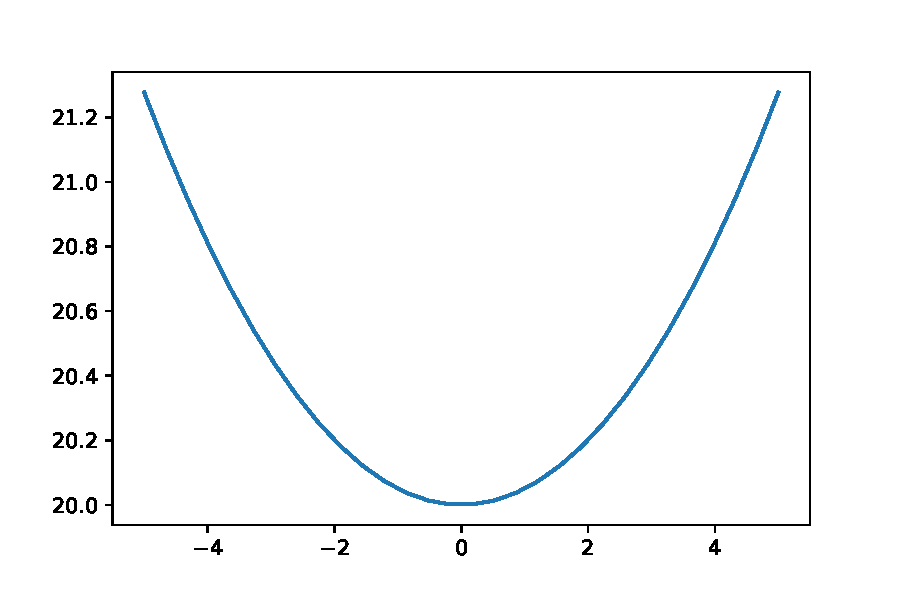
\includegraphics[scale=0.5]{code/fig1}
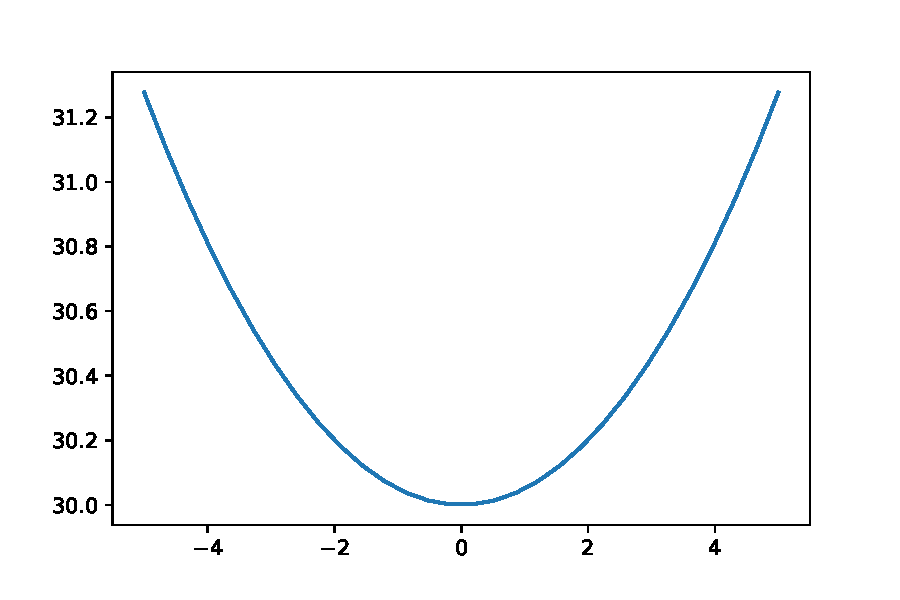
\includegraphics[scale=0.5]{code/fig2}
\caption{Det ses at en ændring fra $h_0=10$ til $h_0=20$ kun ændrer højden af kæden men ikke formen.}
\end{figure}



\begin{figure}[h!]
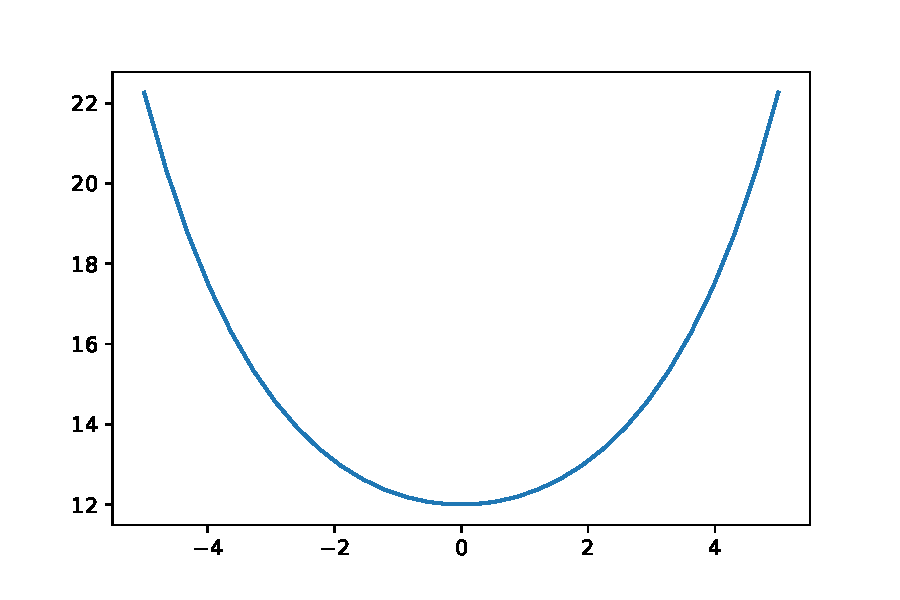
\includegraphics[scale=0.5]{code/fig3}
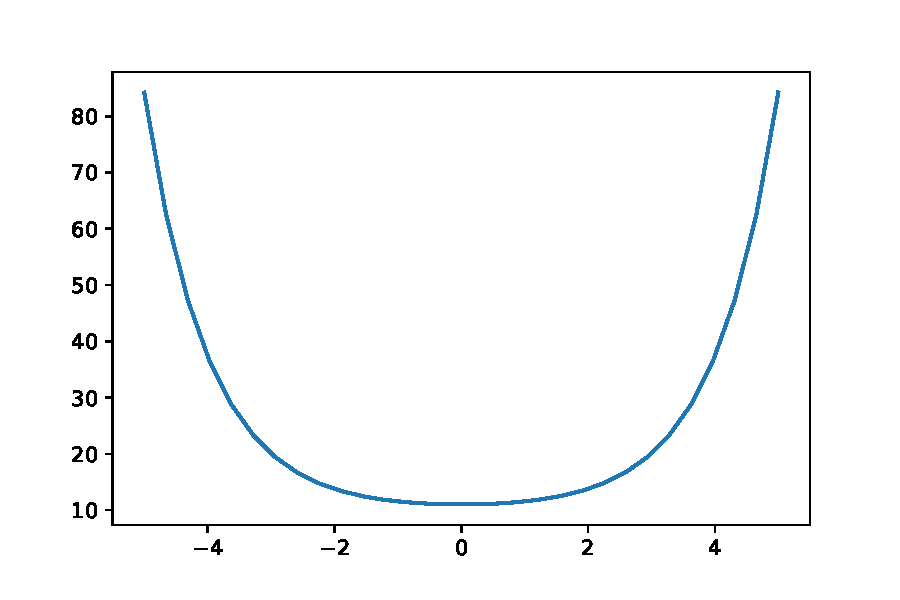
\includegraphics[scale=0.5]{code/fig4}
\caption{Det ses at en ændring fra $\Lambda=2$ til $\lambda=1$ ændrer kædelinjen meget.}
\end{figure}

<<<<<<< HEAD
<<<<<<< HEAD
<<<<<<< HEAD
>>>>>>> master
=======
>>>>>>> master
=======
>>>>>>> master
=======
>>>>>>> master
